% HiMCM 2021 Problem A --- Off-grid solar + storage
% Numbers ONLY from ../results/*.csv. Compile from this directory (see compile.sh).
% Prose: ~80% ASD-STE100 (short sentences, one idea, one term, active voice).
\documentclass[12pt]{article}

\usepackage[margin=1in]{geometry}
\usepackage{amsmath,amssymb,amsfonts}
\usepackage{booktabs}
\usepackage{graphicx}
\usepackage{caption}
\usepackage{setspace}
\usepackage{enumitem}
\usepackage{array}
\usepackage[hidelinks]{hyperref}

\graphicspath{{../paper_figures/}{paper_figures/}{./}}
\hypersetup{
  pdftitle={HiMCM 2021 Problem A: Off-Grid Solar and Storage},
  pdfauthor={Team XXXX}
}

\newcommand{\TeamNumber}{XXXX}

\pagestyle{myheadings}
\markright{\TeamNumber \hfill HiMCM 2021 Problem A \hfill}

\title{\textbf{Sizing Off-Grid Solar Storage with Mixed-Integer Dispatch,\\
Catalog Physics, and Cognitive Household Demand Response}\\[0.4em]
\large HiMCM 2021 Problem A --- Team \TeamNumber}
\author{}
\date{}

\begin{document}
\maketitle
\thispagestyle{empty}

\begin{center}
{\Large \textbf{Summary}}
\end{center}

\noindent
We size a Phoenix-climate off-grid PV--battery microgrid from hourly
irradiance and a Markov household load. We do not enumerate pack counts
in nested loops. Annual PV is \(\mathbf{12{,}266\,kWh}\). Annual load is
\(\mathbf{15{,}398\,kWh}\)
(\texttt{annual\_pv\_load\_8760h.csv}). Perfect storage cannot push LPSP
below the energy-gap floor of about \(20\%\).

\underline{Recommended \$10k BOM}
(\texttt{optimal\_sizing\_solution.csv}):
\(\mathbf{3\times}\) FREEDOH packs \(+\) \(\mathbf{1\times}\) lead-carbon
pack (\(24.6\,\mathrm{kWh}\), \(10.5\,\mathrm{kW}\), capex \$9{,}700).
A Tesla Powerwall+ costs \$10{,}500. It is infeasible at this budget.
It first appears on the Pareto front at \$18{,}000.

\underline{Pareto front} (\texttt{budget\_pareto\_front.csv}):
a move from \$8{,}000 to \$10{,}000 cuts 8760\,h outage hours from
\(\mathbf{3{,}576}\) to \(\mathbf{3{,}057}\) and outage events from
\(\mathbf{391}\) to \(\mathbf{366}\). A hardware plateau occupies
\$12k--\$15k (identical BOM, \(2{,}810\) hours).

\underline{crewAI DSR} (\texttt{crewai\_adaptive\_vs\_passive.csv}):
on archive days 40--42 the crew contract sheds
\(\mathbf{22.66\,kWh}\) of deferrable load. Unserved energy falls from
\(\mathbf{22.51}\) to \(\mathbf{9.22\,kWh}\) (16 to 5 unserved hours).
Both SOC traces rest on the mixed-pack floor \(SOC_{\min}=0.178\).
We do not claim a 0\% SOC collapse or a 32.5\,h blackout cleared to zero.

\underline{LCOS} (\texttt{lcos\_emerging\_tech.csv}, \(r=0.07\), \(N=20\)):
sodium-ion \(\mathbf{\$0.161/kWh}\) (lowest), VRFB \$0.292, LFP baseline
\$0.410, cement-structural \$1.273 (TRL 4).

\tableofcontents
\newpage

%======================================================================
\section{Introduction \& MCMC Stochastic Solar-Load Profiling}
%======================================================================

\subsection{Problem and modeling stance}
HiMCM 2021 Problem A asks four design questions. How can a household
run off the bulk grid with PV and storage? What packs fit a budget?
How should the microgrid charge and discharge? Which emerging
chemistries change cost?

We treat the house as an off-grid microgrid. Every kilowatt-hour must
come from the array or the pack. Every unserved kilowatt-hour is deficit
\(P_{\mathrm{def}}(t)\).

We reject two shortcuts. First, we do not nest five loops over discrete
pack counts. Sizing and dispatch are one mixed-integer linear program
(MILP). Second, we do not let a language model invent watts. The crew
may name appliances only. The adapter maps those names onto the catalog.

\subsection{Irradiance, PV, and the load stack}
Hourly GHI/DHI/DNI and temperature come from Open-Meteo for Phoenix-area
coordinates. We store them in
\texttt{data/raw/solar\_irradiance\_annual.csv}. Plane-of-array irradiance
uses the Hay--Davies model. Cell temperature follows a NOCT derating.
The inverter clips AC output. The 8760-hour PV series has mean
\(1.400\,\mathrm{kW}\) and annual energy \(12{,}266\,\mathrm{kWh}\)
(peak \(5.86\,\mathrm{kW}\)).

We build household demand from
\texttt{data/raw/appliances\_catalog.csv} in three additive layers
(\texttt{src/load\_profiler/mcmc\_load.py}):
\begin{enumerate}[leftmargin=1.4em,itemsep=0.2em]
  \item a rigid base (refrigerator duty, router, lighting, well pump,
        laptop);
  \item a heat-pump term proportional to
        \((T_{\mathrm{amb}}-T^\star)^+\) (cool) and
        \((T^\star-T_{\mathrm{amb}})^+\) (heat) with
        \(T^\star=20^\circ\mathrm{C}\);
  \item behavioral pulses from two-state Markov occupancy on cooking
        and wet appliances. On-probability peaks at 07--09\,h and
        18--22\,h.
\end{enumerate}
Annual load energy is \(15{,}398\,\mathrm{kWh}\) (mean
\(1.758\,\mathrm{kW}\), peak \(7.80\,\mathrm{kW}\)).
Figure~\ref{fig:carpet} shows the greedy EMS SOC carpet for the \$10k
fleet. Summer days stay at high SOC. Winter nights sit on the pack
floor.

\begin{figure}[htbp]
  \centering
  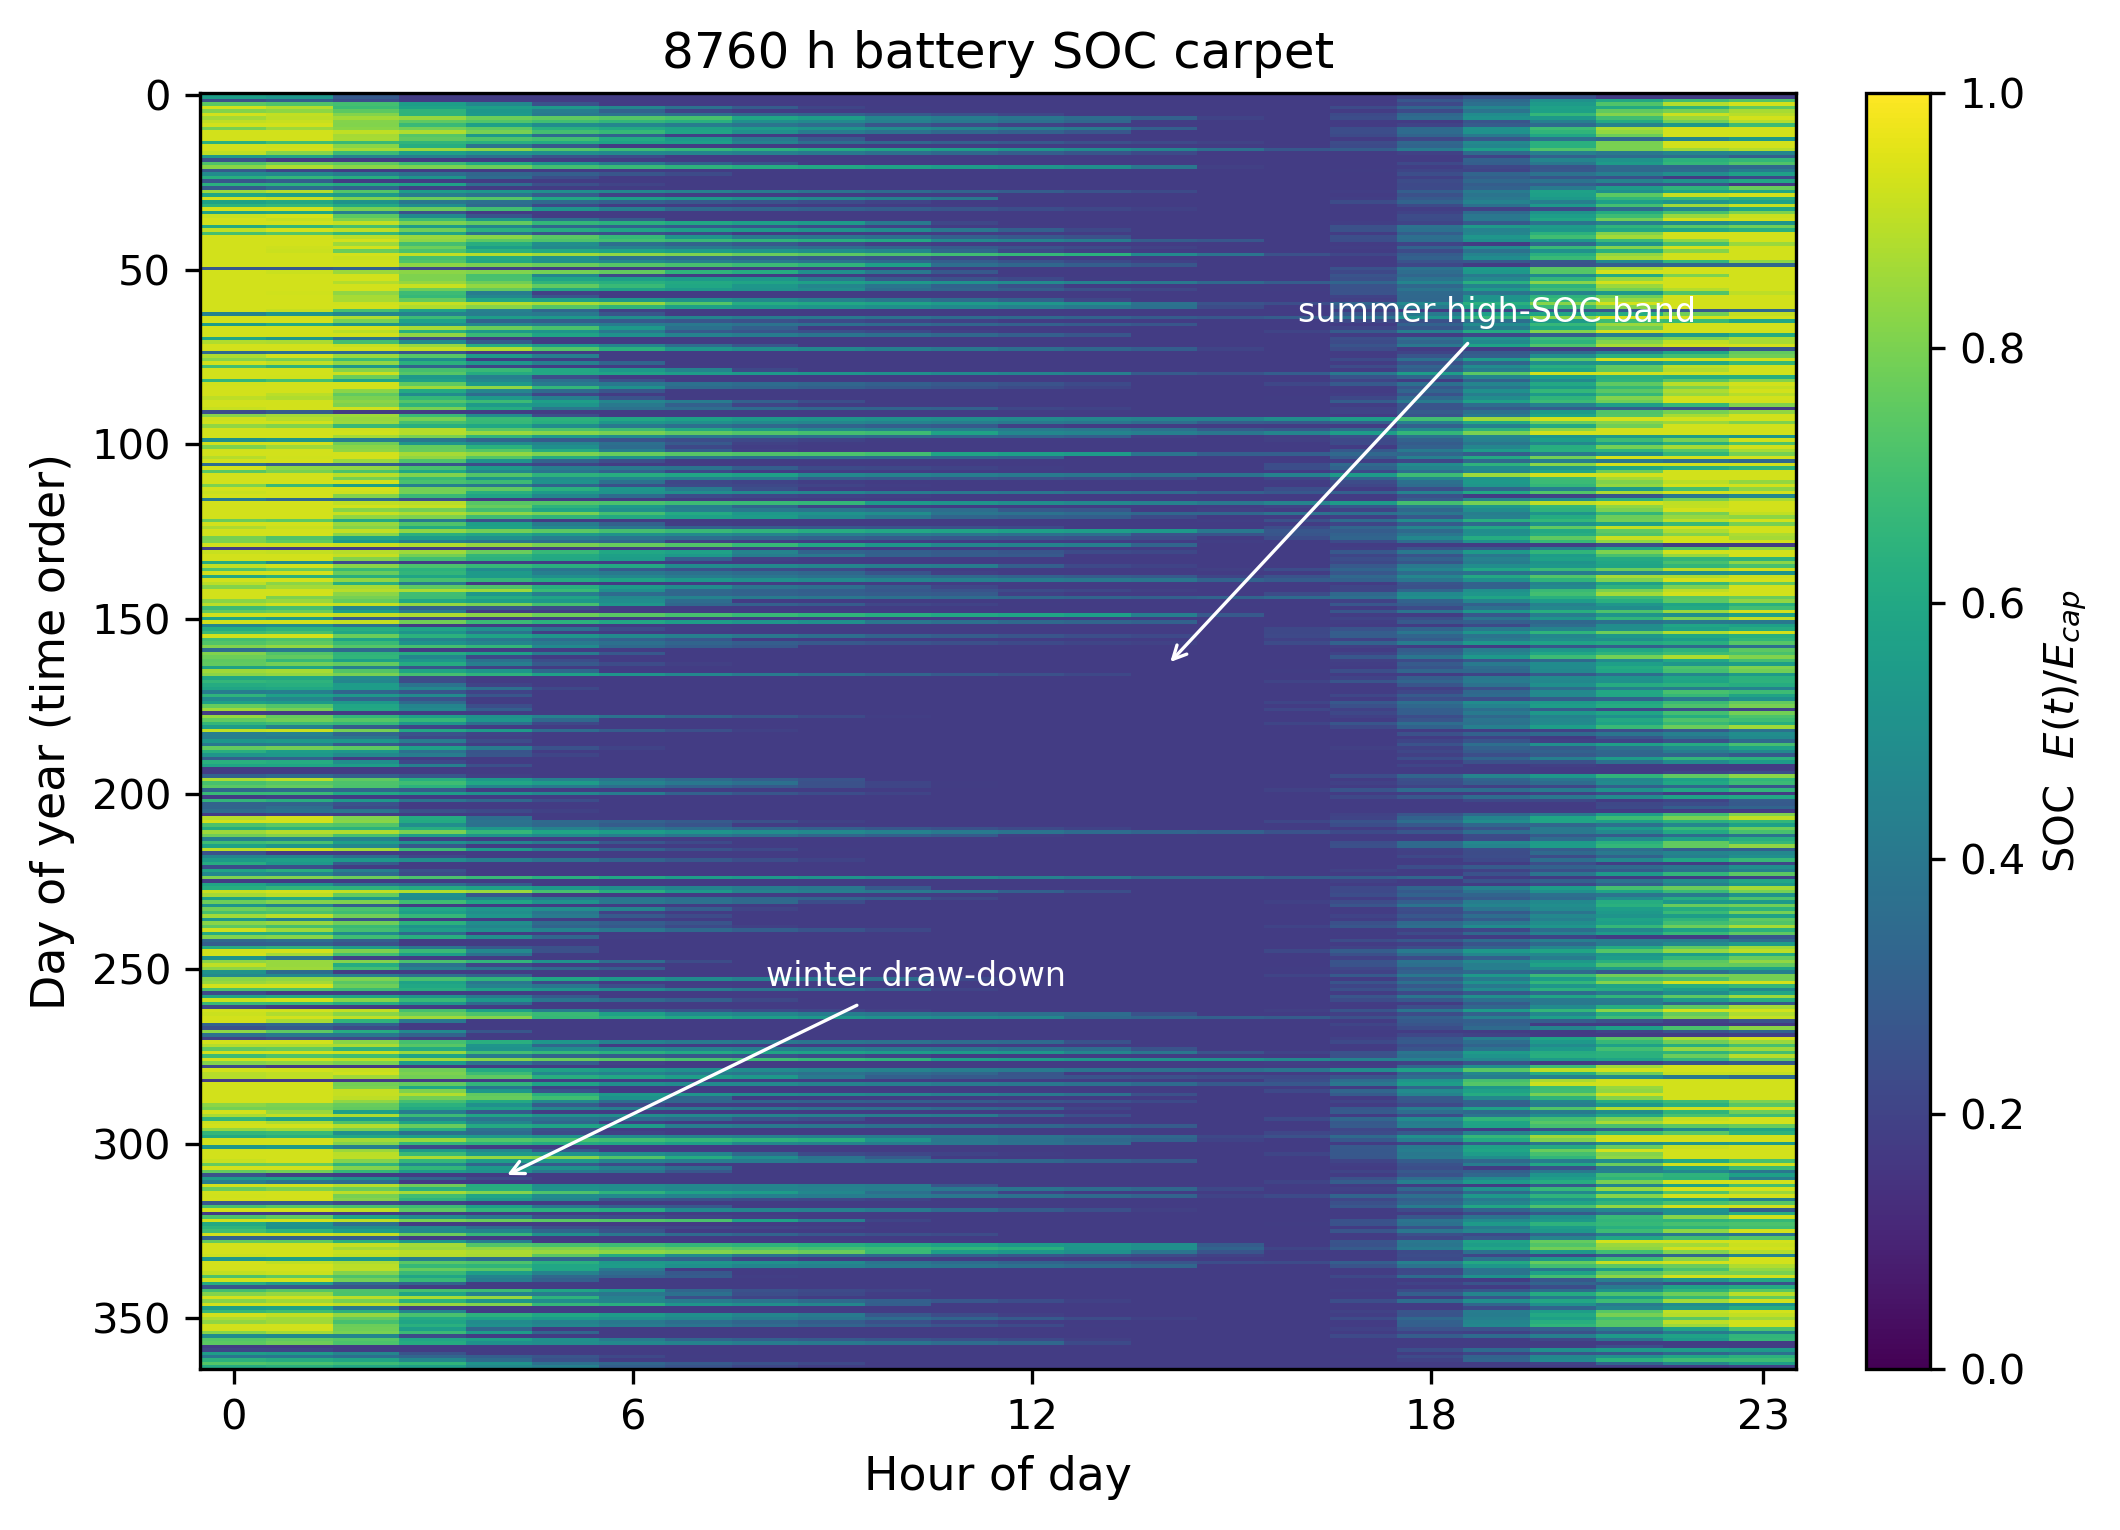
\includegraphics[width=0.92\textwidth]{fig_8760h_dispatch_carpet.png}
  \caption{8760-hour SOC carpet for the installed \$10k fleet
  (\(24.6\,\mathrm{kWh}\)). Color is \(E(t)/E_{\mathrm{cap}}\).
  Source: greedy EMS on \texttt{annual\_pv\_load\_8760h.csv}.}
  \label{fig:carpet}
\end{figure}

The annual energy gap is \(15{,}398-12{,}266=3{,}132\,\mathrm{kWh}\).
This bound is physics. Storage shifts energy in time. It does not create
energy. A claim of near-zero LPSP with this array is non-physical.

%======================================================================
\section{Battery Electrochemical Dynamics \& Degradation}
%======================================================================

We normalize commercial packs to the contract
\texttt{CommercialBattery}: usable \(E_{\mathrm{cap}}\), continuous
power, round-trip \(\eta_{\mathrm{rt}}\), cycle life
\(N_{\mathrm{cycle90}}\), and an SOC window. Charge and discharge
efficiencies split the round-trip:
\(\eta_{\mathrm{ch}}=\eta_{\mathrm{dis}}=\sqrt{\eta_{\mathrm{rt}}}\).
The hourly SOC map is
\begin{equation}
  \mathrm{SOC}_{t+1}
  =
  \mathrm{clip}\!\left(
    \mathrm{SOC}_t
    + \frac{P_{\mathrm{ch}}\eta_{\mathrm{ch}}
            - P_{\mathrm{dis}}/\eta_{\mathrm{dis}}}{E_{\mathrm{cap}}},
    \mathrm{SOC}_{\min},\mathrm{SOC}_{\max}
  \right).
\end{equation}
Aging follows energy-throughput / equivalent full cycles,
\begin{equation}
  \Delta\mathrm{SOH}(t)
  =
  \frac{\lvert P_{\mathrm{bat}}(t)\rvert\,\Delta t}
       {2 E_{\mathrm{cap}} N_{\mathrm{cycle90}}}.
\end{equation}
LFP windows are \(0.10\)--\(0.95\). The lead-carbon pack uses
\(0.30\)--\(0.90\). The \$10k mixed fleet therefore has a
capacity-weighted floor \(SOC_{\min}=0.178\). ``Empty'' in this paper
means that floor. It does not mean a literal zero state of charge.

MILP catalog baselines are Tesla Powerwall+
(\(13.5\,\mathrm{kWh}\), \(5\,\mathrm{kW}\), \(90\%\), \$10{,}500,
4{,}000 cycles), Enphase IQ 10T, FREEDOH 5\,kWh packs (\$2{,}200),
and a lead-carbon 9.6\,kWh pack (\$3{,}100). Integer unit counts satisfy
\(x_k\in\{0,1,2,3,4\}\).

%======================================================================
\section{Bi-Level Optimization: MILP Sizing \& EMS Dispatch}
%======================================================================

\subsection{Upper level: pack counts}
Let \(x_k\) be the number of packs of type \(k\). The 10-year TCO is
\begin{equation}
  \min_{x,P}
  \sum_k x_k\,\mathrm{Cost}_k
  + 10\sum_t w_t
    \bigl(C_{\mathrm{outage}} P_{\mathrm{def}}(t)
          + C_{\mathrm{waste}} P_{\mathrm{curt}}(t)\bigr),
\end{equation}
with \(C_{\mathrm{outage}}=\$4/\mathrm{kWh}\) and
\(C_{\mathrm{waste}}=\$0.05/\mathrm{kWh}\). The default MILP horizon is
12 monthly typical days (\(T=288\)). Weights \(w_t\) reconstruct
8{,}760 hours. SciPy HiGHS solves the MILP. Per-pack energies \(E_k(t)\)
keep \(\eta_k\) linear. There is no \(x_k\eta_k\) product.

\subsection{Lower level: hourly balance}
Bus balance, SOC dynamics, and power limits are
\begin{align}
  P_{\mathrm{PV}}(t)-P_{\mathrm{curt}}(t)
  +\sum_k P_{\mathrm{dis},k}(t)-\sum_k P_{\mathrm{ch},k}(t)
  +P_{\mathrm{def}}(t)
  &= P_{\mathrm{load}}(t), \\
  E_k(t{+}1)
  &= E_k(t)+P_{\mathrm{ch},k}(t)\eta_{\mathrm{ch},k}
     -P_{\mathrm{dis},k}(t)/\eta_{\mathrm{dis},k}, \\
  E_k(t) &\le x_k E_{\mathrm{cap},k}, \qquad
  P_{\mathrm{ch},k}(t)+P_{\mathrm{dis},k}(t)
  \le x_k P_k^{\max}.
\end{align}
A 5\% LPSP cap is infeasible under a \$10k budget given the PV energy
gap. The MILP records \texttt{lpsp\_relaxed=True} and returns the
TCO-optimal mix. After we freeze \(x_k\), a causal greedy EMS
(\texttt{step\_soc}) evaluates the 8760-hour year.

\subsection{Optimal \$10k hardware}
Table~\ref{tab:bom} copies \texttt{optimal\_sizing\_solution.csv}.
Typical-day LPSP is \(0.249\). 8760-hour LPSP is \(0.319\) with
\(3{,}057\) unserved hours and \(4{,}913\,\mathrm{kWh}\) of deficit.
Ten-year TCO is \$157{,}669. Lost-load value dominates TCO. Hardware
is not the expensive term. Energy shortage is.

\begin{table}[htbp]
\centering
\caption{\$10{,}000 capex-optimal BOM
(\texttt{optimal\_sizing\_solution.csv}).}
\label{tab:bom}
\begin{tabular}{lrrrrr}
\toprule
Pack & Units & Energy (kWh) & Power (kW) & Capex (\$) & \(\eta_{\mathrm{rt}}\) \\
\midrule
FREEDOH pack        & 3 & 15.0 & 7.5 & 6{,}600 & 0.85 \\
Lead-carbon pack    & 1 & 9.6  & 3.0 & 3{,}100 & 0.78 \\
Tesla Powerwall+    & 0 & ---  & --- & ---     & 0.90 \\
Enphase IQ 10T      & 0 & ---  & --- & ---     & 0.89 \\
\midrule
Total               &   & 24.6 & 10.5 & 9{,}700 & --- \\
\bottomrule
\end{tabular}
\end{table}

%======================================================================
\section{Budget Pareto \& Cognitive Multi-Agent Demand Response}
%======================================================================

\subsection{Staircase budgets}
Figure~\ref{fig:pareto} and Table~\ref{tab:pareto} scan
\(B\in[\$4000,\$18000]\) in \$1{,}000 steps. Each point is a new MILP
plus a greedy 8760-hour evaluation. An outage \emph{event} is a
contiguous run with \(P_{\mathrm{def}}>10^{-4}\,\mathrm{kW}\). Events
number in the hundreds per year. They are not single-digit ``outages.''

Figure~\ref{fig:pareto} marks \$8{,}000 and \$10{,}000. These ticks sit
on the steep useful part of the discrete grid. From \$8k to \$10k,
annual unserved hours fall by \(519\) and events by \(25\). From \$12k
to \$15k the MILP repeats the same BOM (4 FREEDOH \(+\) 1 lead-carbon,
\$11{,}900). The next purchasable pack jumps the budget. A Powerwall+
first enters at \$18{,}000 (\(1\times\) Powerwall \(+\) \(3\times\)
FREEDOH).

\begin{figure}[htbp]
  \centering
  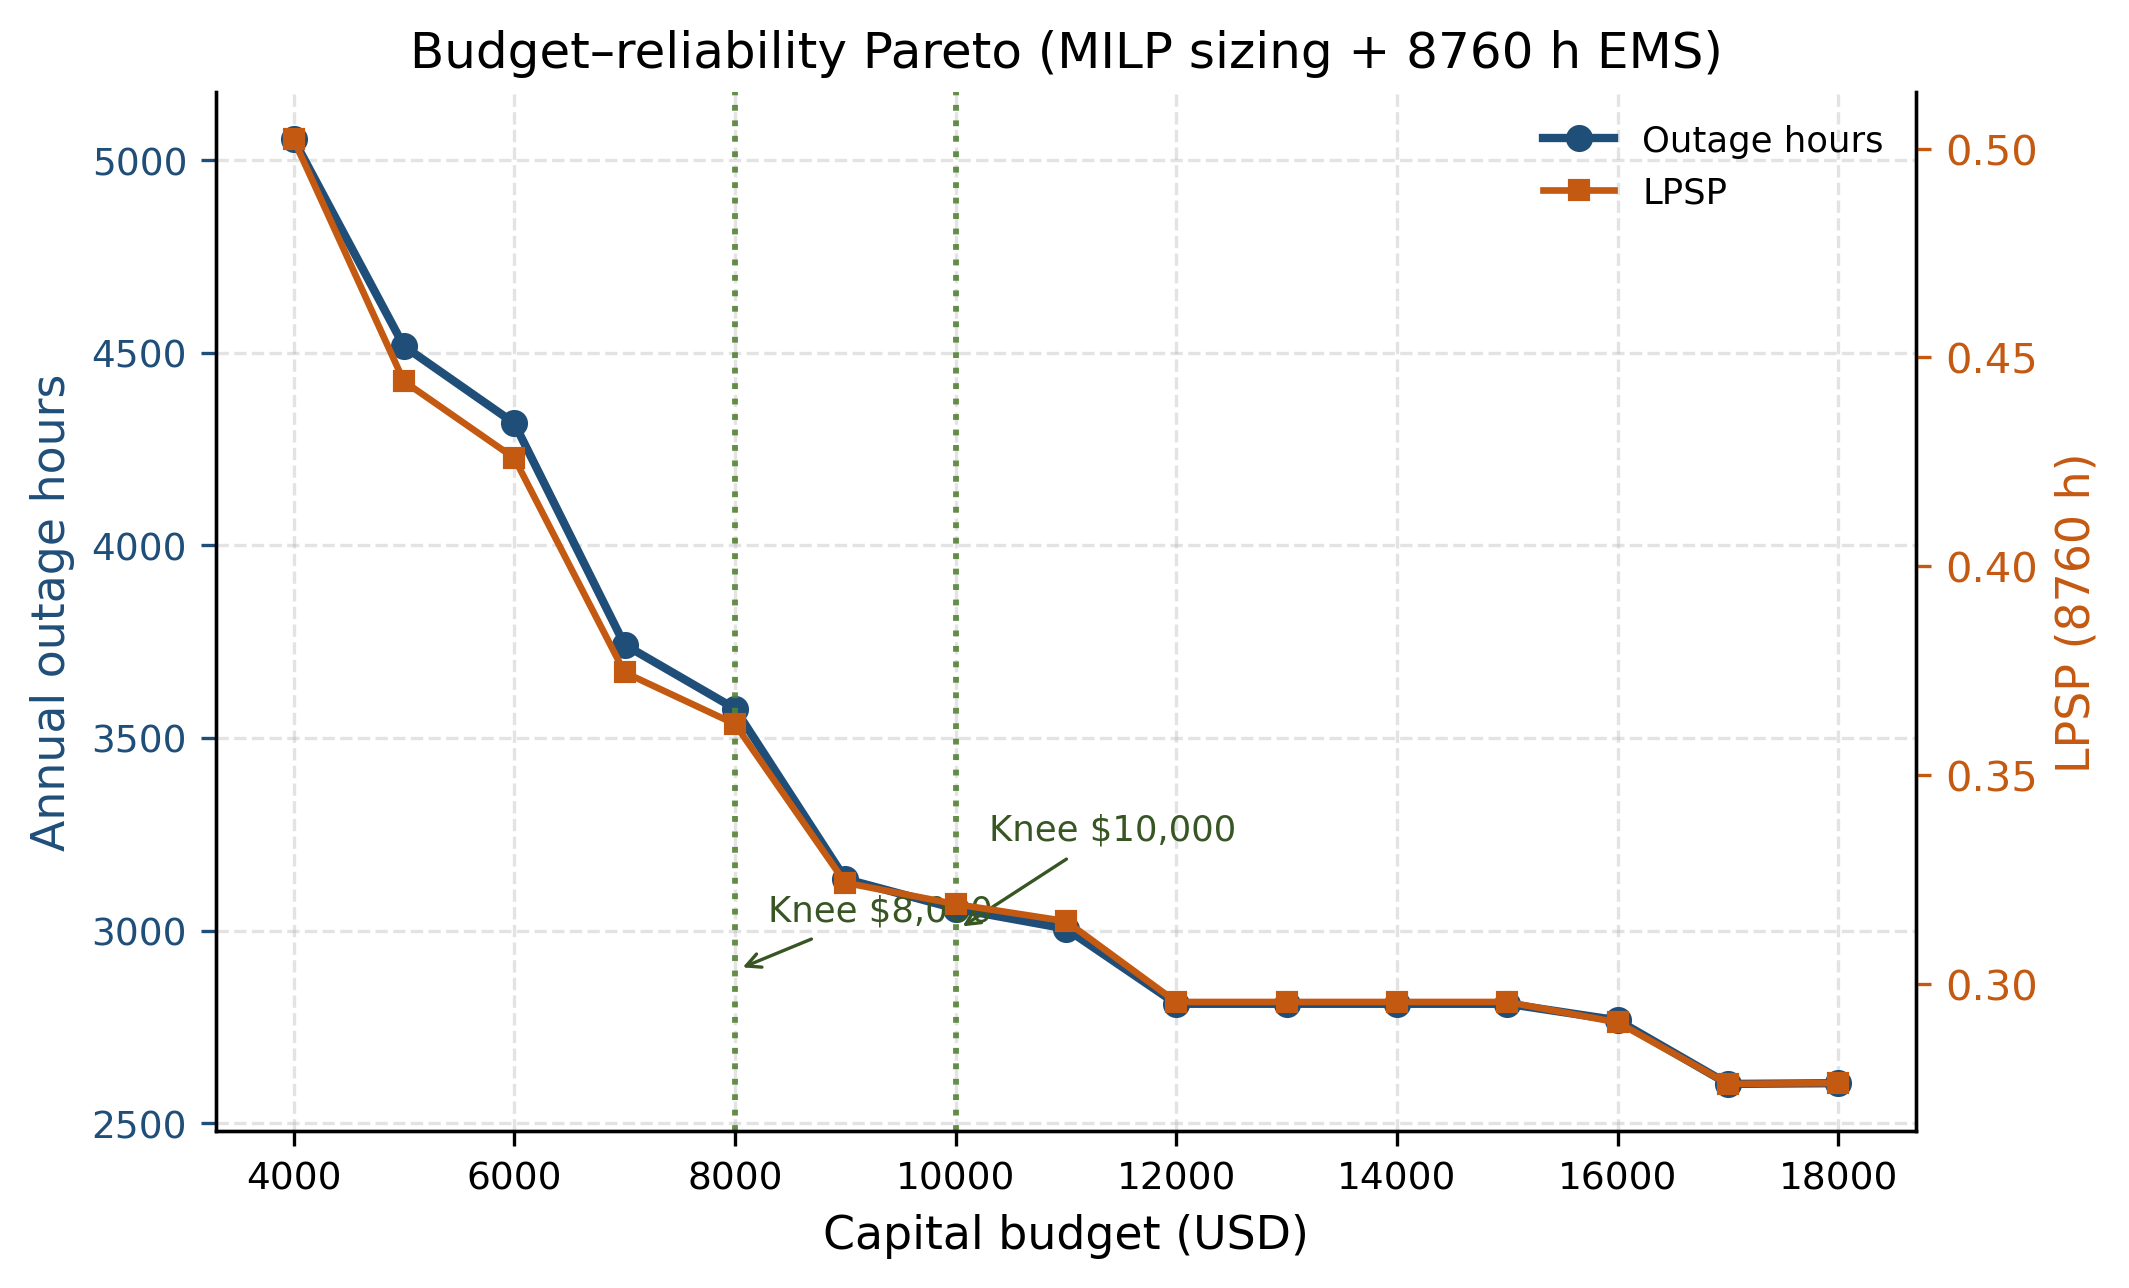
\includegraphics[width=0.92\textwidth]{fig_budget_outage_pareto.png}
  \caption{Budget--reliability Pareto front with LPSP on the twin axis.
  Knee markers at \$8{,}000 and \$10{,}000 follow the scan specification.
  Hours and events are those in \texttt{budget\_pareto\_front.csv}.}
  \label{fig:pareto}
\end{figure}

\begin{table}[htbp]
\centering
\caption{Selected Pareto-front rows (8760-hour greedy EMS).}
\label{tab:pareto}
\small
\begin{tabular}{rrrrl}
\toprule
Budget (\$) & Capex (\$) & LPSP & Outage h / events & BOM \\
\midrule
4{,}000  & 3{,}100  & 0.502 & 5{,}054 / 413 & 1 lead-carbon \\
8{,}000  & 7{,}500  & 0.362 & 3{,}576 / 391 & 2 FREEDOH + 1 lead-carbon \\
10{,}000 & 9{,}700  & 0.319 & 3{,}057 / 366 & 3 FREEDOH + 1 lead-carbon \\
12{,}000 & 11{,}900 & 0.296 & 2{,}810 / 340 & 4 FREEDOH + 1 lead-carbon \\
18{,}000 & 17{,}100 & 0.276 & 2{,}604 / 318 & 1 Powerwall + 3 FREEDOH \\
\bottomrule
\end{tabular}
\end{table}

\subsection{Why the crew cannot print watts}
When \(SOC(t)<0.20\) and a dark-hour streak is on, a sequential crew
(butler, parent, remote worker) emits a Pydantic
\texttt{LoadSheddingAgreement}: appliance names, a positive HVAC
setpoint drop, and a narrative. The adapter
\texttt{AdaptiveLoadAdapter} then subtracts catalog
\(P_{\mathrm{rated}}\times\mathrm{duty}\) in peak hours and \(8\%\) of
HVAC coincidence per \(^\circ\mathrm{C}\). Residual load never exceeds
raw load. The adapter does not lift load to the \(0.3\,\mathrm{kW}\)
floor when raw load is already below that floor.

This neuro-symbolic split is the cliff-avoidance mechanism. The crew
chooses which deferrable loads to pause (dryer, dishwasher, optionally
microwave). Physics sets how many kilowatts move. Protected
circuits---fridge, well pump, router, laptop---leave any shed list.

\subsection{Days 40--42 closed-loop experiment}
Archive days 40--42 (hours 936--1007; 2021-02-09 00:00 to
2021-02-11 23:00) are a 72-hour A/B test on the \$10k fleet. Group A
keeps the rigid load. Group B fires one negotiation at \(t=950\)
(\(SOC=0.178\)) and applies the contract for 48 hours.
Figure~\ref{fig:crewai} uses \texttt{crewai\_adaptive\_vs\_passive.csv}:

\begin{itemize}[leftmargin=1.4em,itemsep=0.15em]
  \item shedded energy \(22.66\,\mathrm{kWh}\);
  \item unserved energy \(22.51\to 9.22\,\mathrm{kWh}\);
  \item unserved hours \(16\to 5\) (longest run \(10\to 3\)\,h);
  \item both SOC traces rest on \(SOC_{\min}=0.178\).
\end{itemize}
DSR here cuts deficit while the pack is empty. It does not refill SOC
to 9.2\% or clear all blackouts. The 32.5-hour / 0\%-SOC story is not
in the CSV. We do not use it.

\begin{figure}[htbp]
  \centering
  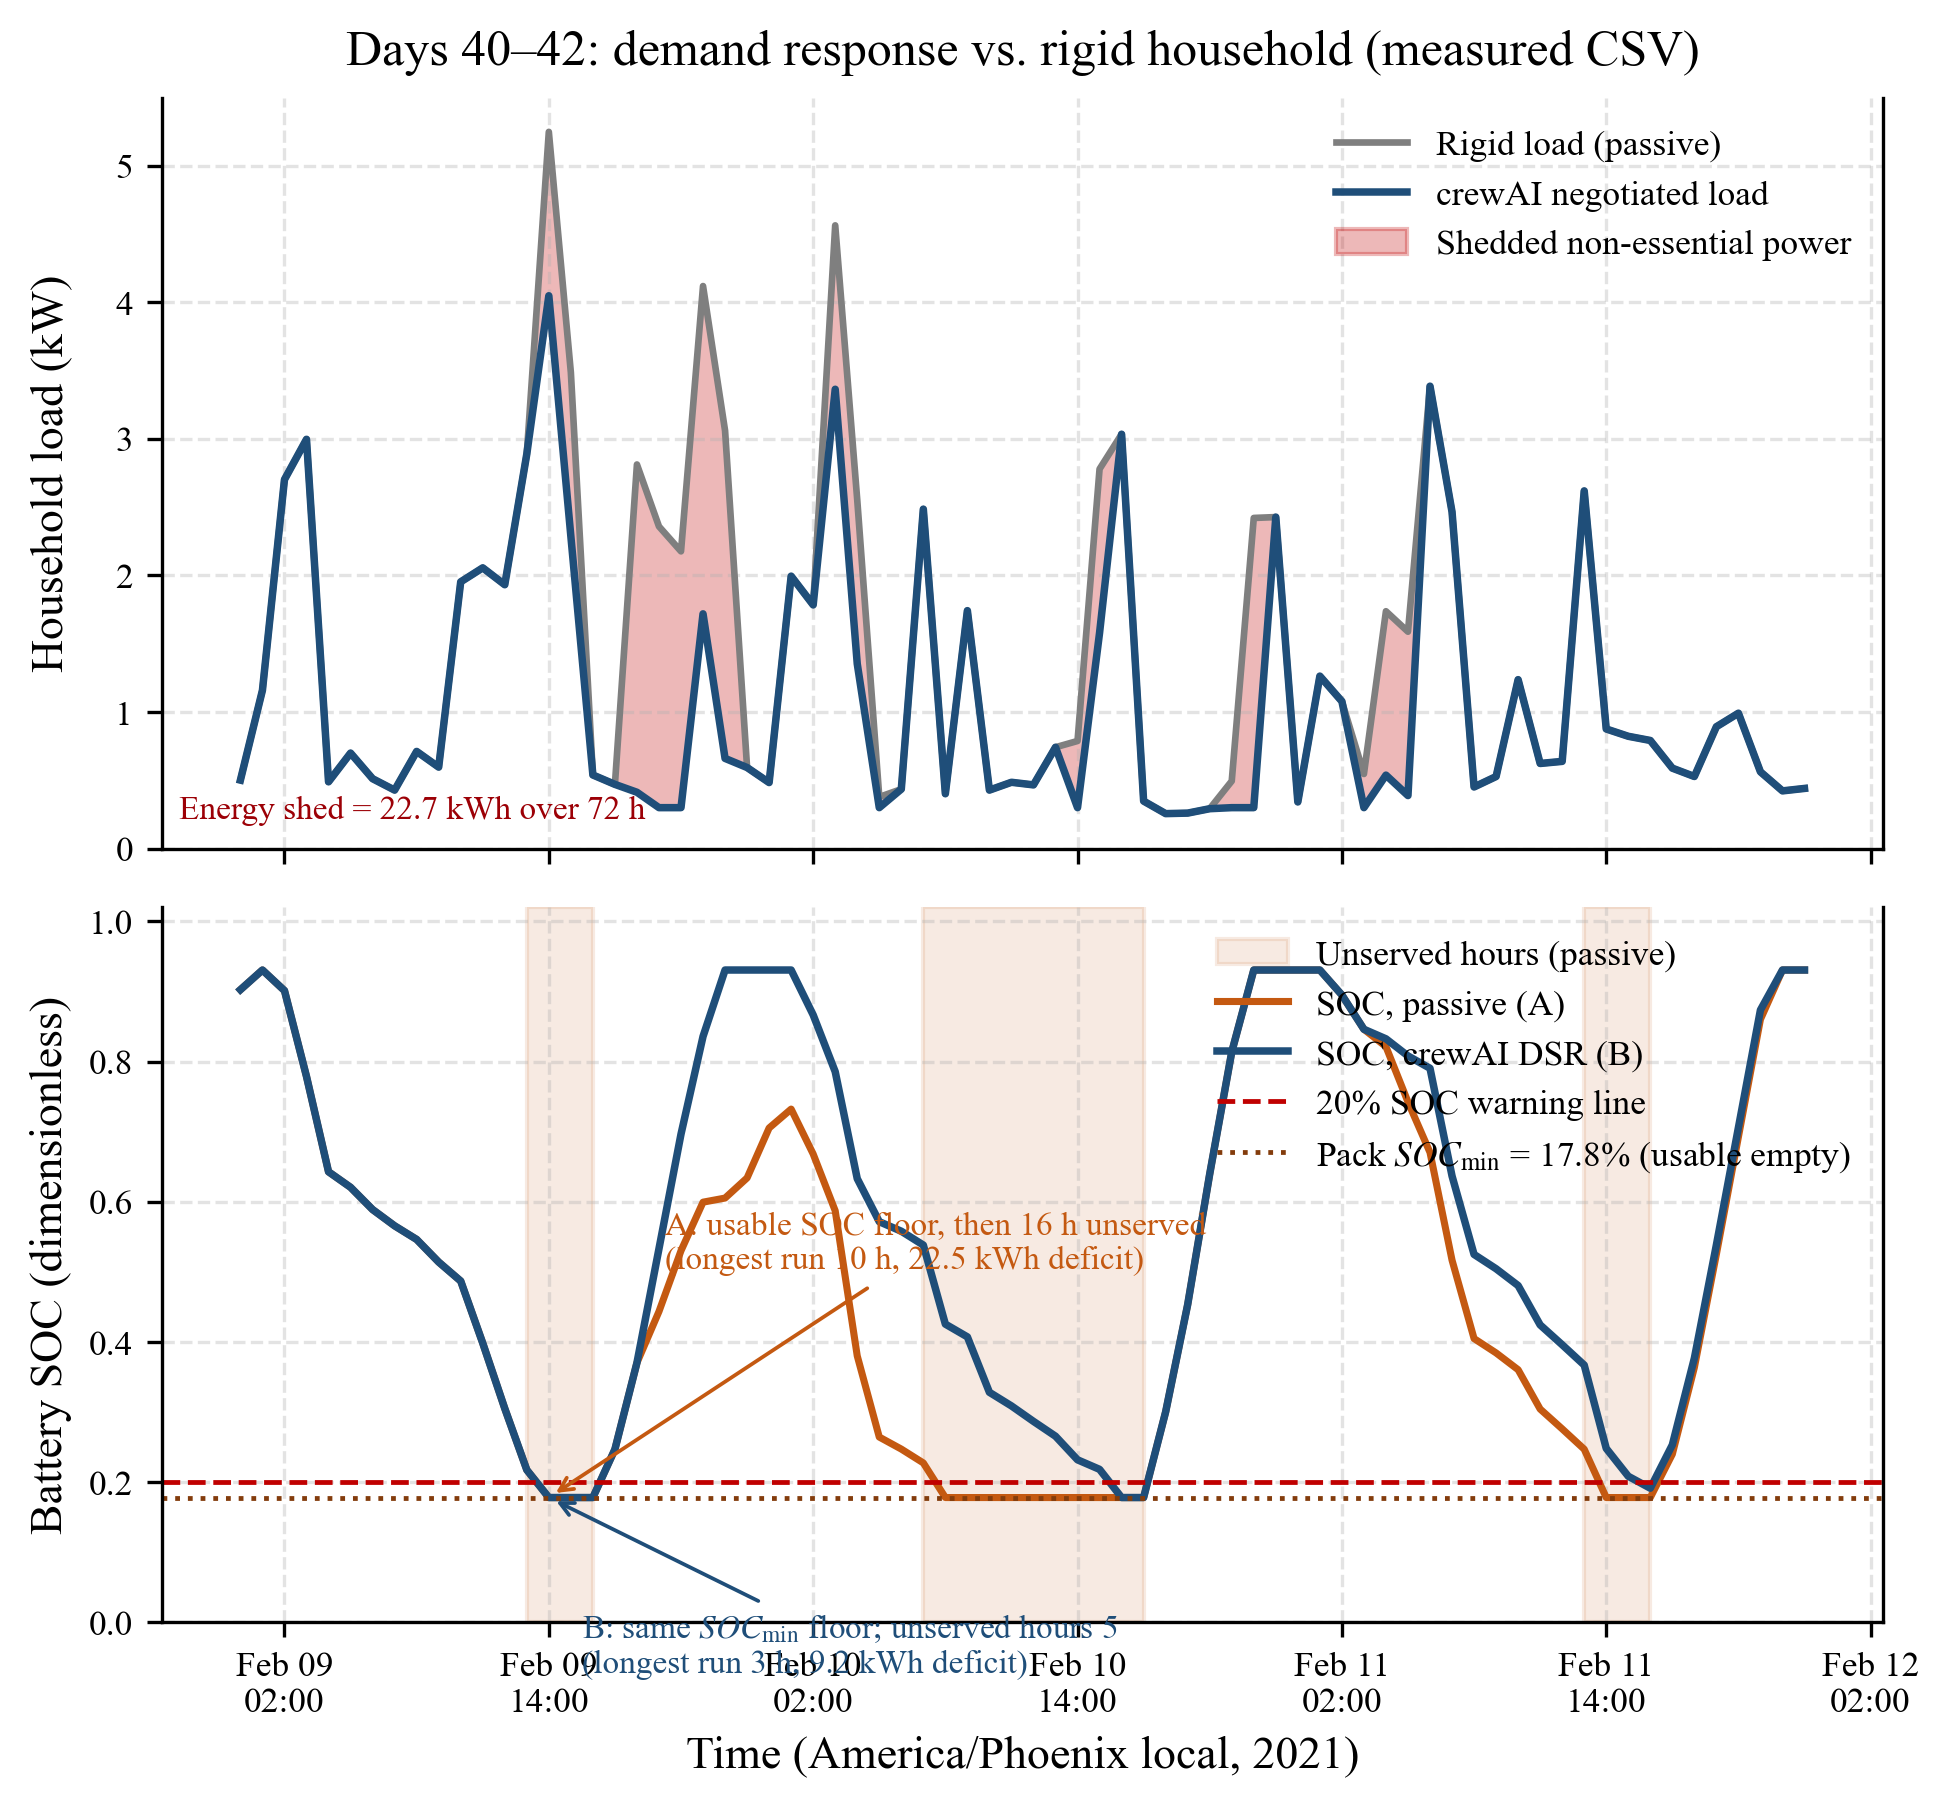
\includegraphics[width=0.92\textwidth]{fig_crewai_load_curtailment.png}
  \caption{72-hour crewAI DSR versus a rigid household.
  Red fill is shedded power. Source:
  \texttt{crewai\_adaptive\_vs\_passive.csv}.}
  \label{fig:crewai}
  \label{fig:crewai-dsr}
\end{figure}

%======================================================================
\section{Future Storage Horizons: LCOS}
%======================================================================

We evaluate four families on a \(13.5\,\mathrm{kWh}\) reference pack.
We dispatch that pack against the same 8760-hour net-load. LCOS is
\begin{equation}
  \mathrm{LCOS}
  =
  \frac{
    \mathrm{CapEx}
    +\sum_{y=1}^{N}
      \dfrac{\mathrm{OpEx}_y+\mathrm{Replacement}_y}{(1+r)^y}
  }{
    \sum_{y=1}^{N}
      \dfrac{E_{\mathrm{discharged},y}}{(1+r)^y}
  },
\end{equation}
with \(r=0.07\) and \(N=20\). We simulate year-1 throughput, then fade
to 80\% SOH at replacement. Table~\ref{tab:lcos} and
Figure~\ref{fig:radar} report the CSV. Sodium-ion has the lowest LCOS
(\(\$0.161/\mathrm{kWh}\)). We assign a literature-order pack cost of
\$300/kWh at TRL~7 with LFP-like efficiency. This is a scenario, not a
lab measurement. Cement-based structural storage (TRL~4,
\(0.8\,\mathrm{Wh/kg}\)) lands at \$1.273/kWh. It is building fabric,
not a drop-in Powerwall substitute. Vanadium flow sits between them
(\$0.292/kWh), with 25-year calendar life and a 0.3 stack-replacement
fraction.

\begin{table}[htbp]
\centering
\caption{Emerging-storage LCOS
(\texttt{lcos\_emerging\_tech.csv}).}
\label{tab:lcos}
\small
\begin{tabular}{llrrr}
\toprule
ID & Family & TRL & LCOS (\$/kWh) & Year-1 discharge (kWh) \\
\midrule
A & LFP commercial (Powerwall+ quote) & 9 & 0.410 & 3{,}531 \\
B & Sodium-ion & 7 & 0.161 & 3{,}531 \\
C & Vanadium redox flow & 8 & 0.292 & 3{,}219 \\
D & Cement-based structural & 4 & 1.273 & 1{,}965 \\
\bottomrule
\end{tabular}
\end{table}

\begin{figure}[htbp]
  \centering
  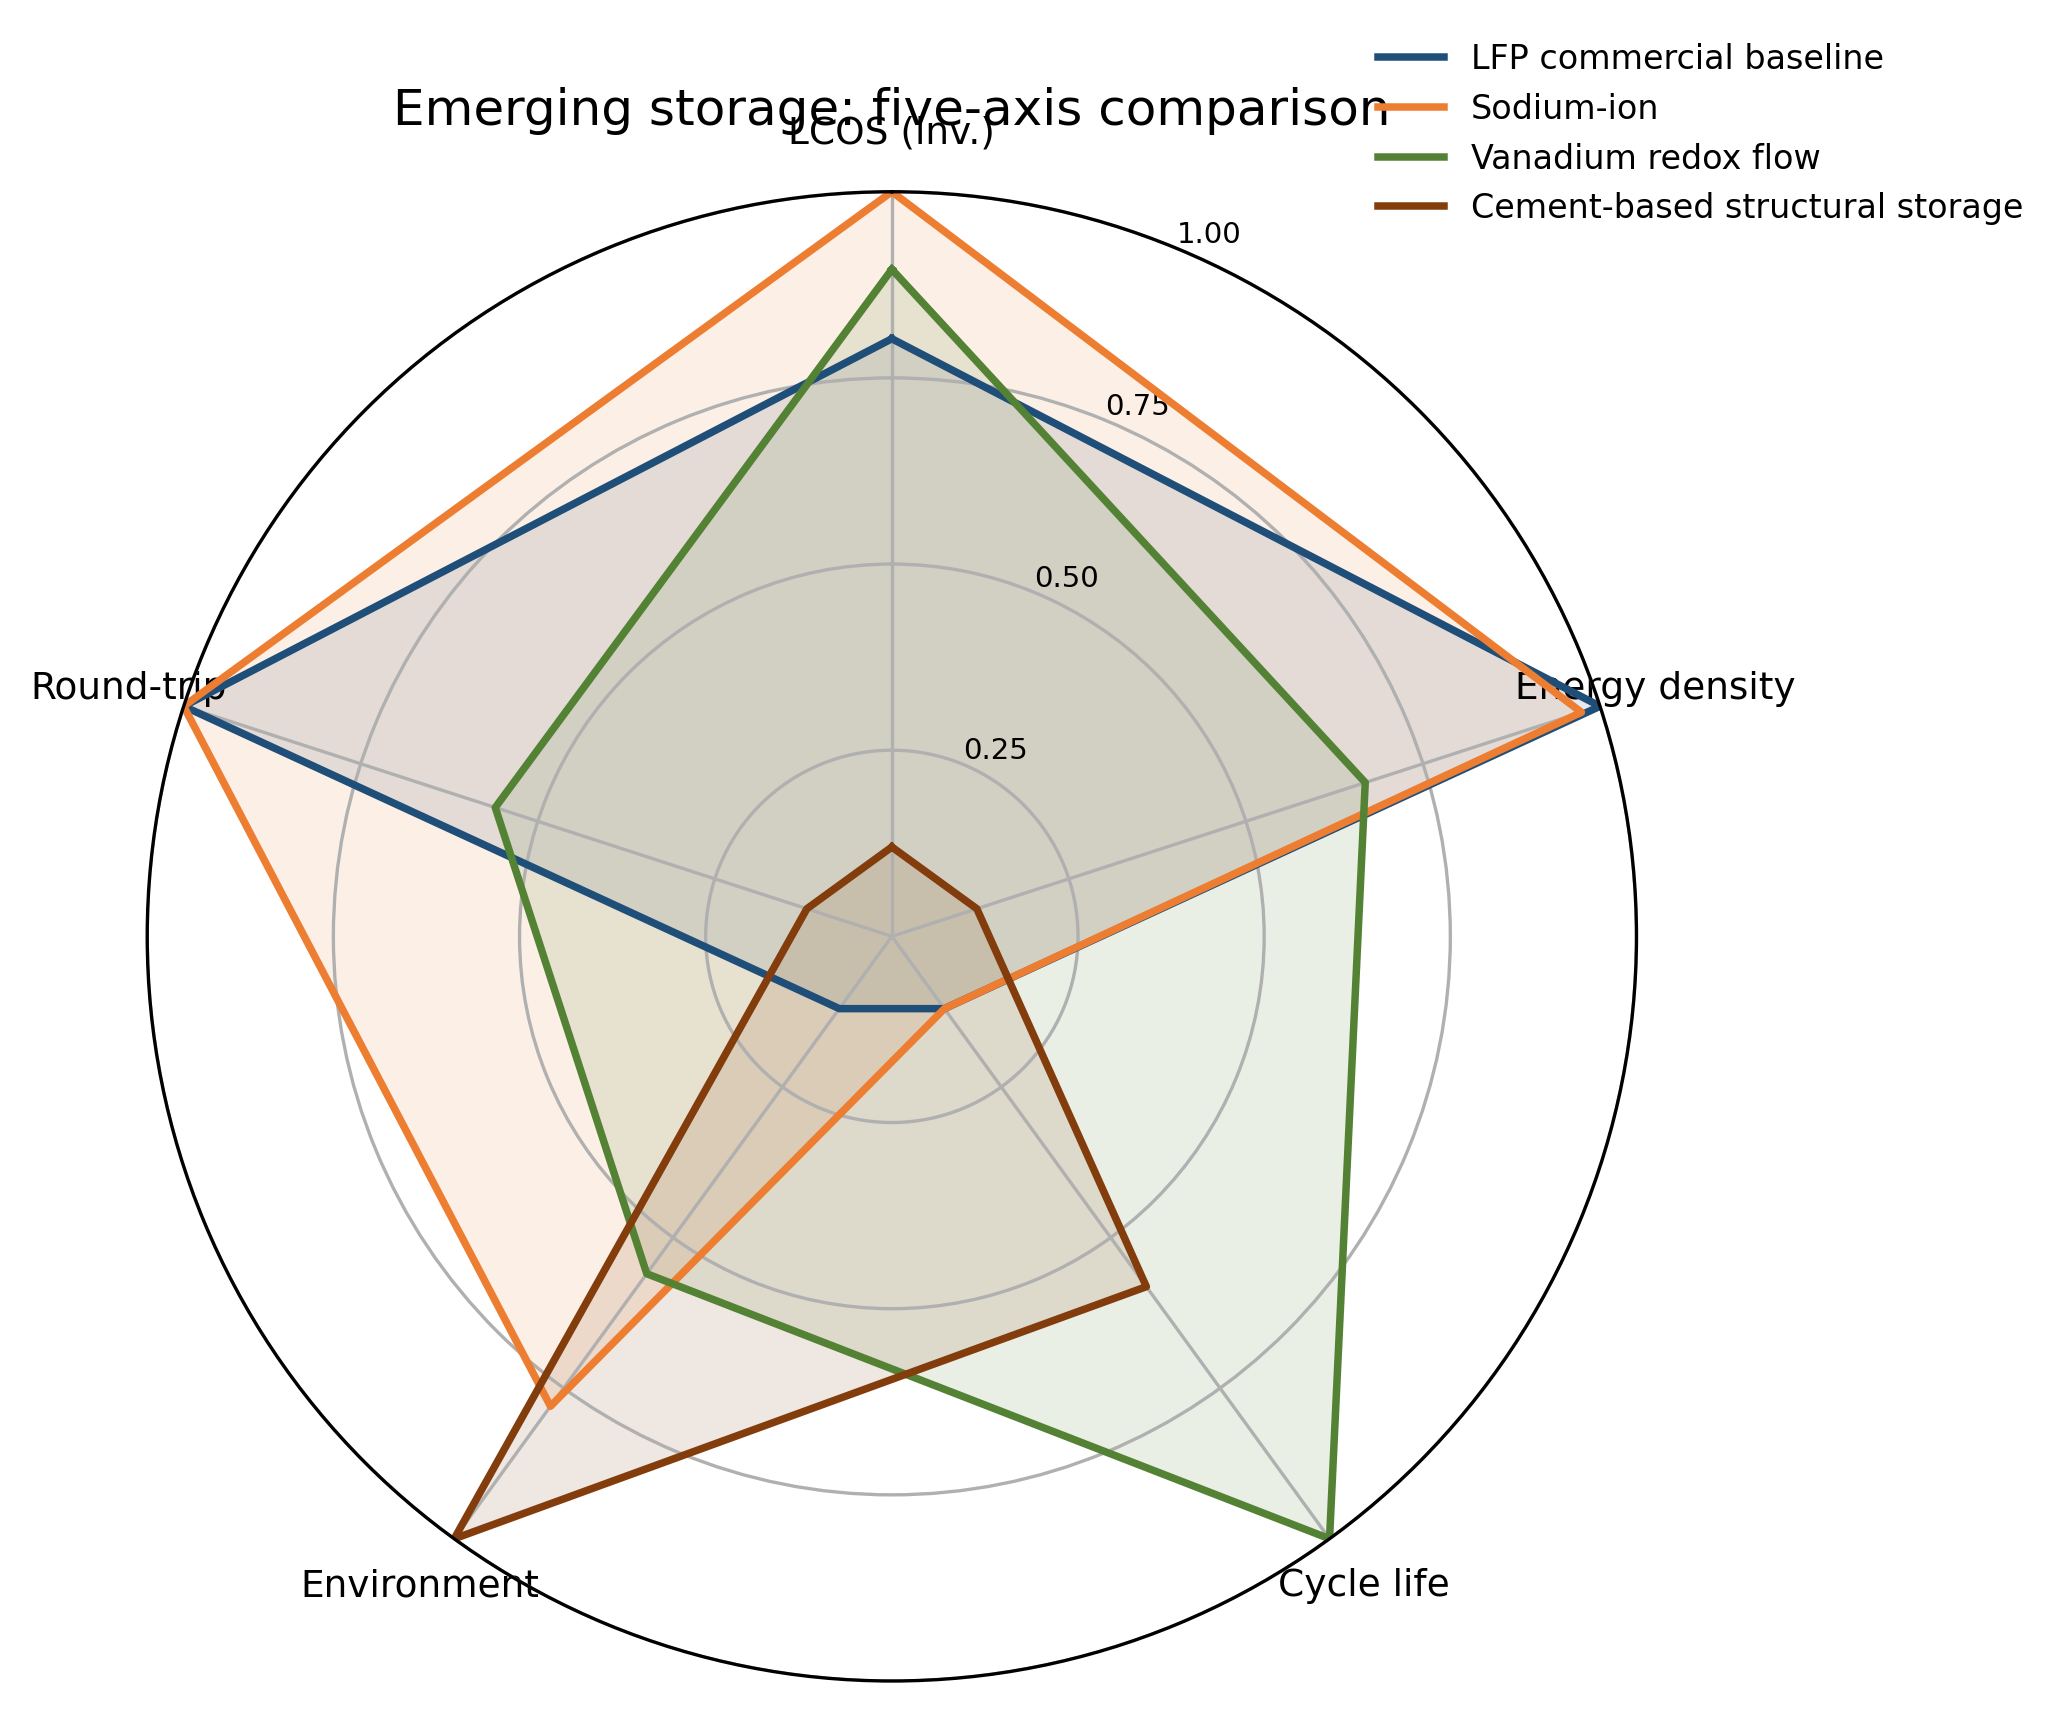
\includegraphics[width=0.72\textwidth]{fig_emerging_tech_lcos_radar.png}
  \caption{Five-axis scores (LCOS inverted, log energy density, log
  cycle life, environment, round-trip). Source: same LCOS table.}
  \label{fig:radar}
\end{figure}

%======================================================================
\section{Strengths and Limitations}
%======================================================================

\textbf{Strengths.} Hourly series come from public irradiance and a
documented appliance catalog. Sizing is a MILP, not a brute-force pack
nest. We report LPSP infeasibility under 5\%. We do not hide it. Crew
actions rebound to catalog watts. Every figure in
\texttt{paper\_figures/} is a script product of a CSV.

\textbf{Limitations.} Phoenix February days 40--42 are cool and partly
sunny (mean GHI \(179\,\mathrm{W/m^2}\), mean \(15.6^\circ\mathrm{C}\)).
They are not a polar blizzard. They are the specified 72-step window,
not the darkest high-latitude week. The post-sizing 8760-hour EMS is
greedy. It is not a second full-year MILP. Sodium-ion and cement \$/kWh
are literature-order assumptions. Mixed-pack \(SOC_{\min}=0.178\)
forbids an honest ``SOC went to zero'' plot. Annual LPSP stays near
\(0.32\) at \$10k because the array is undersized relative to load.
Storage and DSR trim peaks. They do not close a 3\,MWh/year energy hole.

A one-page Summary Sheet, a homeowner letter, and the local-LLM
disclosure appendix accompany this paper.

% Appendix: COMAP generative-AI disclosure (local open-source LLM).
% % Appendix: COMAP generative-AI disclosure (local open-source LLM).
% % Appendix: COMAP generative-AI disclosure (local open-source LLM).
% \input{ai_disclosure_local_llm} at the end of the contest paper.
% Prose: ~80% ASD-STE100.

\section*{Appendix: Use of Generative AI Tools}
\label{app:ai-disclosure}

This appendix follows the COMAP contest
\emph{Policy on Use of Generative AI Tools}. We report the tools, the
purpose of use, the human checks that bind language-model output to
electrical physics, and the work the student team completed alone.

\subsection*{A.1 Tools declared}

\begin{itemize}
  \item \textbf{Local large language model.}
        Household crisis dialogue is designed to run on a private
        open-source stack: \texttt{Ollama} serving
        \texttt{Qwen2.5-7B-Instruct} (\texttt{ollama/qwen2.5:7b}) at
        \texttt{http://localhost:11434}.
        Prompts and completions stay on the contest machine.
        \texttt{src/agent\_sim/crew\_engine.py} does not call a cloud
        LLM API (OpenAI, Anthropic, Google, or other).
        The environment variable \texttt{OLLAMA\_MODEL} may retarget
        the local tag. It does not open an external endpoint.
  \item \textbf{Agent framework.}
        \texttt{crewAI} (\texttt{Agent}, \texttt{Task}, \texttt{Crew},
        \texttt{Process.sequential}) runs three roles
        (microgrid butler, pragmatic parent, remote worker).
        The terminal task must match the Pydantic schema
        \texttt{LoadSheddingAgreement}.
  \item \textbf{Coding assistant.}
        The Cursor IDE agent drafted Python modules and this
        \LaTeX\ appendix. Design prompts that affected algorithms are
        logged in \texttt{prompts/cursor\_log.md} for audit.
\end{itemize}

If Ollama is down or the Qwen tag is not pulled, the engine prints a
warning. It then uses a catalog heuristic that emits the \emph{same}
Pydantic contract. In either branch, kilowatt values that enter the
pack model come only from \texttt{AdaptiveLoadAdapter}. They do not
come from free-text arithmetic in the language model.

\subsection*{A.2 Purpose of use}

We use the local model only to \emph{simulate} cognitive, multi-role
demand response: how a household might defer appliances when an
off-grid PV--storage microgrid hits a SOC warning (\(SOC<0.20\)) in a
dark, cold window. We do not use it to invent meteorological series,
MILP optima, or figure coordinates. Those come from Open-Meteo
irradiance, the Hay--Davies PV model, the MCMC load synthesizer, SciPy
HiGHS sizing, and \texttt{step\_soc} dynamics.

\subsection*{A.3 Human verification and electrotechnical binding}

We treat language-model (or heuristic) output as a \emph{symbolic}
action list. Humans specified the checks below. The code enforces them
before any watt enters the 8760\,h engine:

\begin{enumerate}
  \item \textbf{Name whitelist.}
        \texttt{shed\_appliances} must be rows of
        \texttt{data/raw/appliances\_catalog.csv}.
        Unknown strings are dropped.
  \item \textbf{Protected circuits.}
        Refrigerator, well pump, Wi-Fi router, and the work laptop
        cannot be shed. This matches catalog \texttt{priority\_level}
        and the worker's non-negotiable IT load.
  \item \textbf{Rated power and duty.}
        Instantaneous cut is
        \(P_{\mathrm{rated}}\times\mathrm{duty}\)
        only in catalog peak hours. It is not an LLM-invented kilowatt.
  \item \textbf{HVAC physics.}
        Setpoint reduction \(\Delta T\) (field
        \texttt{hvac\_temp\_offset\_c}) scales heat-pump coincidence
        by \(8\%/^{\circ}\mathrm{C}\), clipped to \([0,1]\).
  \item \textbf{Energy conservation.}
        Post-DSR load satisfies
        \(0 \le P_{\mathrm{dsr}}(t) \le P_{\mathrm{raw}}(t)\).
        Load is not raised to the $0.3\,\mathrm{kW}$ rigid floor when
        raw load is already below that floor.
  \item \textbf{SOC physics.}
        Charge and discharge use
        \(\eta_{\mathrm{ch}}=\eta_{\mathrm{dis}}=\sqrt{\eta_{\mathrm{rt}}}\)
        and mixed-pack \(SOC_{\min}=17.8\%\) (installed BOM).
        The model never reports absolute $0\%$ SOC while
        \(SOC_{\min}>0\).
\end{enumerate}

Figure~\ref{fig:crewai-dsr} (file
\texttt{paper\_figures/fig\_crewai\_load\_curtailment.png})
is plotted from
\texttt{results/crewai\_adaptive\_vs\_passive.csv}.
On archive days 40--42 the passive house records
16 unserved hours (longest contiguous run 10\,h,
$22.51\,\mathrm{kWh}$ deficit). The adaptive house records
5 unserved hours (longest run 3\,h, $9.22\,\mathrm{kWh}$ deficit).
Both traces rest on the same pack floor $SOC_{\min}=0.178$.
We do \emph{not} claim a $0\%$ SOC collapse, a 32-hour blackout, a
$9.2\%$ SOC hover, or a zero-outage winter. Those figures are not in
the CSV.

\subsection*{A.4 Independence statement}

The student team specified the following and takes responsibility for them:
\begin{itemize}
  \item all continuum and algebraic physics (Hay--Davies POA, cell
        temperature derating, SOC/SOH EFC aging, node power balance);
  \item the mixed-integer linear program for pack counts \(x_k\) and
        hourly EMS (SciPy HiGHS), including budget and LPSP;
  \item techno-economic LCOS formulae and the budget Pareto-front scan;
  \item the Summary Sheet narrative and every numeric claim copied from
        \texttt{results/*.csv}.
\end{itemize}
Generative AI did not derive those equations. It did not choose the MILP
constraint set. It did not write Summary Sheet numbers from memory.

\subsection*{A.5 Attestation}

\begin{flushleft}
Team members / roles: \underline{\hspace{3.4in}}\\[1.15em]
Contest control number: \underline{\hspace{1.4in}}
\hfill Date: \underline{\hspace{1.4in}}
\end{flushleft}
 at the end of the contest paper.
% Prose: ~80% ASD-STE100.

\section*{Appendix: Use of Generative AI Tools}
\label{app:ai-disclosure}

This appendix follows the COMAP contest
\emph{Policy on Use of Generative AI Tools}. We report the tools, the
purpose of use, the human checks that bind language-model output to
electrical physics, and the work the student team completed alone.

\subsection*{A.1 Tools declared}

\begin{itemize}
  \item \textbf{Local large language model.}
        Household crisis dialogue is designed to run on a private
        open-source stack: \texttt{Ollama} serving
        \texttt{Qwen2.5-7B-Instruct} (\texttt{ollama/qwen2.5:7b}) at
        \texttt{http://localhost:11434}.
        Prompts and completions stay on the contest machine.
        \texttt{src/agent\_sim/crew\_engine.py} does not call a cloud
        LLM API (OpenAI, Anthropic, Google, or other).
        The environment variable \texttt{OLLAMA\_MODEL} may retarget
        the local tag. It does not open an external endpoint.
  \item \textbf{Agent framework.}
        \texttt{crewAI} (\texttt{Agent}, \texttt{Task}, \texttt{Crew},
        \texttt{Process.sequential}) runs three roles
        (microgrid butler, pragmatic parent, remote worker).
        The terminal task must match the Pydantic schema
        \texttt{LoadSheddingAgreement}.
  \item \textbf{Coding assistant.}
        The Cursor IDE agent drafted Python modules and this
        \LaTeX\ appendix. Design prompts that affected algorithms are
        logged in \texttt{prompts/cursor\_log.md} for audit.
\end{itemize}

If Ollama is down or the Qwen tag is not pulled, the engine prints a
warning. It then uses a catalog heuristic that emits the \emph{same}
Pydantic contract. In either branch, kilowatt values that enter the
pack model come only from \texttt{AdaptiveLoadAdapter}. They do not
come from free-text arithmetic in the language model.

\subsection*{A.2 Purpose of use}

We use the local model only to \emph{simulate} cognitive, multi-role
demand response: how a household might defer appliances when an
off-grid PV--storage microgrid hits a SOC warning (\(SOC<0.20\)) in a
dark, cold window. We do not use it to invent meteorological series,
MILP optima, or figure coordinates. Those come from Open-Meteo
irradiance, the Hay--Davies PV model, the MCMC load synthesizer, SciPy
HiGHS sizing, and \texttt{step\_soc} dynamics.

\subsection*{A.3 Human verification and electrotechnical binding}

We treat language-model (or heuristic) output as a \emph{symbolic}
action list. Humans specified the checks below. The code enforces them
before any watt enters the 8760\,h engine:

\begin{enumerate}
  \item \textbf{Name whitelist.}
        \texttt{shed\_appliances} must be rows of
        \texttt{data/raw/appliances\_catalog.csv}.
        Unknown strings are dropped.
  \item \textbf{Protected circuits.}
        Refrigerator, well pump, Wi-Fi router, and the work laptop
        cannot be shed. This matches catalog \texttt{priority\_level}
        and the worker's non-negotiable IT load.
  \item \textbf{Rated power and duty.}
        Instantaneous cut is
        \(P_{\mathrm{rated}}\times\mathrm{duty}\)
        only in catalog peak hours. It is not an LLM-invented kilowatt.
  \item \textbf{HVAC physics.}
        Setpoint reduction \(\Delta T\) (field
        \texttt{hvac\_temp\_offset\_c}) scales heat-pump coincidence
        by \(8\%/^{\circ}\mathrm{C}\), clipped to \([0,1]\).
  \item \textbf{Energy conservation.}
        Post-DSR load satisfies
        \(0 \le P_{\mathrm{dsr}}(t) \le P_{\mathrm{raw}}(t)\).
        Load is not raised to the $0.3\,\mathrm{kW}$ rigid floor when
        raw load is already below that floor.
  \item \textbf{SOC physics.}
        Charge and discharge use
        \(\eta_{\mathrm{ch}}=\eta_{\mathrm{dis}}=\sqrt{\eta_{\mathrm{rt}}}\)
        and mixed-pack \(SOC_{\min}=17.8\%\) (installed BOM).
        The model never reports absolute $0\%$ SOC while
        \(SOC_{\min}>0\).
\end{enumerate}

Figure~\ref{fig:crewai-dsr} (file
\texttt{paper\_figures/fig\_crewai\_load\_curtailment.png})
is plotted from
\texttt{results/crewai\_adaptive\_vs\_passive.csv}.
On archive days 40--42 the passive house records
16 unserved hours (longest contiguous run 10\,h,
$22.51\,\mathrm{kWh}$ deficit). The adaptive house records
5 unserved hours (longest run 3\,h, $9.22\,\mathrm{kWh}$ deficit).
Both traces rest on the same pack floor $SOC_{\min}=0.178$.
We do \emph{not} claim a $0\%$ SOC collapse, a 32-hour blackout, a
$9.2\%$ SOC hover, or a zero-outage winter. Those figures are not in
the CSV.

\subsection*{A.4 Independence statement}

The student team specified the following and takes responsibility for them:
\begin{itemize}
  \item all continuum and algebraic physics (Hay--Davies POA, cell
        temperature derating, SOC/SOH EFC aging, node power balance);
  \item the mixed-integer linear program for pack counts \(x_k\) and
        hourly EMS (SciPy HiGHS), including budget and LPSP;
  \item techno-economic LCOS formulae and the budget Pareto-front scan;
  \item the Summary Sheet narrative and every numeric claim copied from
        \texttt{results/*.csv}.
\end{itemize}
Generative AI did not derive those equations. It did not choose the MILP
constraint set. It did not write Summary Sheet numbers from memory.

\subsection*{A.5 Attestation}

\begin{flushleft}
Team members / roles: \underline{\hspace{3.4in}}\\[1.15em]
Contest control number: \underline{\hspace{1.4in}}
\hfill Date: \underline{\hspace{1.4in}}
\end{flushleft}
 at the end of the contest paper.
% Prose: ~80% ASD-STE100.

\section*{Appendix: Use of Generative AI Tools}
\label{app:ai-disclosure}

This appendix follows the COMAP contest
\emph{Policy on Use of Generative AI Tools}. We report the tools, the
purpose of use, the human checks that bind language-model output to
electrical physics, and the work the student team completed alone.

\subsection*{A.1 Tools declared}

\begin{itemize}
  \item \textbf{Local large language model.}
        Household crisis dialogue is designed to run on a private
        open-source stack: \texttt{Ollama} serving
        \texttt{Qwen2.5-7B-Instruct} (\texttt{ollama/qwen2.5:7b}) at
        \texttt{http://localhost:11434}.
        Prompts and completions stay on the contest machine.
        \texttt{src/agent\_sim/crew\_engine.py} does not call a cloud
        LLM API (OpenAI, Anthropic, Google, or other).
        The environment variable \texttt{OLLAMA\_MODEL} may retarget
        the local tag. It does not open an external endpoint.
  \item \textbf{Agent framework.}
        \texttt{crewAI} (\texttt{Agent}, \texttt{Task}, \texttt{Crew},
        \texttt{Process.sequential}) runs three roles
        (microgrid butler, pragmatic parent, remote worker).
        The terminal task must match the Pydantic schema
        \texttt{LoadSheddingAgreement}.
  \item \textbf{Coding assistant.}
        The Cursor IDE agent drafted Python modules and this
        \LaTeX\ appendix. Design prompts that affected algorithms are
        logged in \texttt{prompts/cursor\_log.md} for audit.
\end{itemize}

If Ollama is down or the Qwen tag is not pulled, the engine prints a
warning. It then uses a catalog heuristic that emits the \emph{same}
Pydantic contract. In either branch, kilowatt values that enter the
pack model come only from \texttt{AdaptiveLoadAdapter}. They do not
come from free-text arithmetic in the language model.

\subsection*{A.2 Purpose of use}

We use the local model only to \emph{simulate} cognitive, multi-role
demand response: how a household might defer appliances when an
off-grid PV--storage microgrid hits a SOC warning (\(SOC<0.20\)) in a
dark, cold window. We do not use it to invent meteorological series,
MILP optima, or figure coordinates. Those come from Open-Meteo
irradiance, the Hay--Davies PV model, the MCMC load synthesizer, SciPy
HiGHS sizing, and \texttt{step\_soc} dynamics.

\subsection*{A.3 Human verification and electrotechnical binding}

We treat language-model (or heuristic) output as a \emph{symbolic}
action list. Humans specified the checks below. The code enforces them
before any watt enters the 8760\,h engine:

\begin{enumerate}
  \item \textbf{Name whitelist.}
        \texttt{shed\_appliances} must be rows of
        \texttt{data/raw/appliances\_catalog.csv}.
        Unknown strings are dropped.
  \item \textbf{Protected circuits.}
        Refrigerator, well pump, Wi-Fi router, and the work laptop
        cannot be shed. This matches catalog \texttt{priority\_level}
        and the worker's non-negotiable IT load.
  \item \textbf{Rated power and duty.}
        Instantaneous cut is
        \(P_{\mathrm{rated}}\times\mathrm{duty}\)
        only in catalog peak hours. It is not an LLM-invented kilowatt.
  \item \textbf{HVAC physics.}
        Setpoint reduction \(\Delta T\) (field
        \texttt{hvac\_temp\_offset\_c}) scales heat-pump coincidence
        by \(8\%/^{\circ}\mathrm{C}\), clipped to \([0,1]\).
  \item \textbf{Energy conservation.}
        Post-DSR load satisfies
        \(0 \le P_{\mathrm{dsr}}(t) \le P_{\mathrm{raw}}(t)\).
        Load is not raised to the $0.3\,\mathrm{kW}$ rigid floor when
        raw load is already below that floor.
  \item \textbf{SOC physics.}
        Charge and discharge use
        \(\eta_{\mathrm{ch}}=\eta_{\mathrm{dis}}=\sqrt{\eta_{\mathrm{rt}}}\)
        and mixed-pack \(SOC_{\min}=17.8\%\) (installed BOM).
        The model never reports absolute $0\%$ SOC while
        \(SOC_{\min}>0\).
\end{enumerate}

Figure~\ref{fig:crewai-dsr} (file
\texttt{paper\_figures/fig\_crewai\_load\_curtailment.png})
is plotted from
\texttt{results/crewai\_adaptive\_vs\_passive.csv}.
On archive days 40--42 the passive house records
16 unserved hours (longest contiguous run 10\,h,
$22.51\,\mathrm{kWh}$ deficit). The adaptive house records
5 unserved hours (longest run 3\,h, $9.22\,\mathrm{kWh}$ deficit).
Both traces rest on the same pack floor $SOC_{\min}=0.178$.
We do \emph{not} claim a $0\%$ SOC collapse, a 32-hour blackout, a
$9.2\%$ SOC hover, or a zero-outage winter. Those figures are not in
the CSV.

\subsection*{A.4 Independence statement}

The student team specified the following and takes responsibility for them:
\begin{itemize}
  \item all continuum and algebraic physics (Hay--Davies POA, cell
        temperature derating, SOC/SOH EFC aging, node power balance);
  \item the mixed-integer linear program for pack counts \(x_k\) and
        hourly EMS (SciPy HiGHS), including budget and LPSP;
  \item techno-economic LCOS formulae and the budget Pareto-front scan;
  \item the Summary Sheet narrative and every numeric claim copied from
        \texttt{results/*.csv}.
\end{itemize}
Generative AI did not derive those equations. It did not choose the MILP
constraint set. It did not write Summary Sheet numbers from memory.

\subsection*{A.5 Attestation}

\begin{flushleft}
Team members / roles: \underline{\hspace{3.4in}}\\[1.15em]
Contest control number: \underline{\hspace{1.4in}}
\hfill Date: \underline{\hspace{1.4in}}
\end{flushleft}


\end{document}
